% ==========================================================================
% The Modeling Decision: report skeleton (6 pages max, refs + AI appendix excluded)
%
% REQUIREMENT CHECKLIST (comments only, not printed)
%  R1 decision, who decides, cost of each error type ........ Sec. 1
%  R2 baseline declared before modeling, shown beside number . Sec. 2, 5
%  R3 simple model + flexible model, same split and metric ... Sec. 3
%  R4 unsupervised structure that CHANGES the decision ........ Sec. 4
%  R5 failure analysis: >=2 slice variables, n + interval,
%     worst slice named, exploratory slices marked ............ Sec. 6
%  R6 recommendation + the one fact that would reverse it ..... Sec. 7
%  Locked items (split, metric, baseline): any change must be declared in
%  Sec. 2 "Declared changes" with a reason.
%  Repo: README with exact command for the headline number, fixed seed,
%  data included or fetched by script.
%
%  Rubric warning: if a heading could have been written before seeing the
%  data, rename it into a claim once results are in.
% ==========================================================================
\documentclass[11pt]{article}
\usepackage[margin=1in]{geometry}
\usepackage{amsmath,amssymb}
\usepackage{booktabs}
\usepackage{graphicx}
\usepackage{xcolor}
\usepackage{enumitem}
\usepackage[colorlinks=true,linkcolor=black,citecolor=black,urlcolor=blue]{hyperref}
\setlist{itemsep=1pt,topsep=2pt}

% red placeholder; delete every  before submitting

\title{{Limitations of Univariate Time-Series Data for Forecasting Traffic Slowdowns at Maritime Chokepoints}}
\author{{Sam Whitney} \\ CSCI 5622, Fall 2026}
\date{November, 15th 2026}

\begin{document}
\maketitle

\begin{abstract}

    As recent events have made clear, disruptions to commercial maritime travel can be costly and have wide ranging consequences. Statistical modelling for maritime traffic is a complex problem, as it is difficult to account for the complex systems of global trade, weather, and geopolitical events simultaneously. 
    
    The present work attempted to approach this challenge using a simple logistic regression model applied to a single variable, number of ships per day, calculated at 28 global maritime chokepoints. 

    The decision the model is meant to assist in making is whether to reroute ships bound for chokepoint waterways based on the predicted probability of a traffic slowdown occuring at the waterway in the next seven days. A likely slowdown at a given chokepoint is flagged  if the model predicts a drop below 70\% of the previous 28 day average in the next 7 days.  The metric used to validate model predictions is Recall with a budget of $K=3$ (Recall@3), meaning the top 3 most likely chokepoints to experience a slowdown in the forecasted period are reviwed. 

    The data for the experiment was downloaded in compliance with the IMF license for published work \cite{imfterms}, and consists of multiple date or location aligned datasets from \url{PortWatch.org} \cite{portwatch}, combined into a single univariate panel time-series dataset, split chronologically at January 1st, 2025. Data from before the split date was used for training, and data from after was used for the test set. A logistic regression on three scale-free ratio features \textbf{achieved 0.824, against a persistence baseline of 0.527}. That model was compared against gradient boosting, which showed no significant improvement. 

    However, further exploratory analysis of results confirmed that this headline recall is responding primarily to noise in the dataset. The three chokepoints with traffic below 10 ships per day carried 45\% of the positive tests, and 54\% of alert instances. Excluding those, the model achieves Recall@3 of 0.799 against the 0.609 baseline, with the worst slice in the data coming from two high-traffic lanes for which the model predicted none of the 44 slowdowns in 2025. 

    Neither model is recommended for use outside of a research context, and for further research on the same data Logistic Regression is recommended for the interpretability of its output. 

    GitHub \url{https://github.com/samAmabile/Maritime}


    
\end{abstract}

% --------------------------------------------------------------------------
\section{The decision and the data}  % R1   (~0.75 page)
% --------------------------------------------------------------------------
\paragraph{Decision.}
A shipping risk analyst for a supplier of commodities reporting risk assessments for all planned routes in the coming week has to calculate the risk of sending ships through one of multiple chokepoints required for the cargo to reach its destination. 
A missed slowdown costs money, time, and could potentially jeopardize delivery of time-sensitive cargo, or at worst cause damage to vessels and loss of life. A false alarm costs money and time for expensive reroutes, but as long as the cargo reaches its destingation in an acceptable amount of time the worst consequences can be avoided. \textbf{Sending ships into a potentially high-risk situation resulting from a blockage, closure, or weather event in a narrow waterway must be avoided, even at the cost of some unnecessary and costly reroutes.}  

\paragraph{Data provenanve and terms.}
Daily ship transit counts for $|\mathcal{C}|=28$ chokepoints, 2019-01-01 to 2026-10-18 ($N=79{,}744$ chokepoint-days, complete panel \cite{alam}, no duplicates) from IMF PortWatch. Source: International Monetary Fund, PortWatch. \emph{Daily Chokepoint Transit Calls and Trade Volume Estimates}, \url{https://portwatch.imf.org/pages/data-and-methodology}, downloaded October, 2026. The counts are modeled estimates of vessels transiting 28 chokepoint waterways derived from AIS signals, not official confirmed transits. PortWatch revises the full dataset when there is a change in vessel coverage, chokepoint boundaries, or spoofing checks. The most recent update was in August 2026. All project results use the data downloaded in October 2026. Used under the IMF's terms for published statistical data. All features, lables, and models presented here are the authors own transformations of data downloaded from PortWatch and are not IMF products nor do they carry any endorsement from the IMF. The data are provided 'as is' with no warranty \cite{imfterms}. 

We use only the total daily count $x_{c,t}$.

\paragraph{Target.}
Let $\mu^{(28)}_{c,t}$ be the mean of $x_{c,t-1},\dots,x_{c,t-28}$ and $F_{c,t}$ the mean of $x_{c,t+1},\dots,x_{c,t+7}$. A \emph{slowdown} is
\begin{equation}
y_{c,t} = \mathbf{1}\!\left[F_{c,t} < 0.7\,\mu^{(28)}_{c,t}\right].
\end{equation}
Positives are rare ($\approx 3\%$ of rows) and clustered in a few chokepoints. 

\paragraph{Features and baseline.}
Features use only days $t-28,\dots,t-1$. With $\mu^{(7)}_{c,t}$ the 7-day mean, $\mu^{(28)}_{c,t}$ the 28-day mean, and $\sigma^{(28)}_{c,t}$ the 28-day standard deviation, the model inputs are scale-free ratios
\[
r^{(7/28)}_{c,t}=\frac{\mu^{(7)}_{c,t}}{\mu^{(28)}_{c,t}},\quad
r^{L}_{c,t}=\frac{x_{c,t-1}}{\mu^{(28)}_{c,t}},\quad
\mathrm{cv}_{c,t}=\frac{\sigma^{(28)}_{c,t}}{\mu^{(28)}_{c,t}},
\]
defined when $\mu^{(28)}_{c,t}>0$ (rows with a zero baseline are excluded). Ratios are used because the label is relative and raw traffic levels drift. The persistence baseline scores a row $s_{c,t}=1-r^{(7/28)}_{c,t}$: the further recent traffic already sits below baseline, the higher the score

% --------------------------------------------------------------------------
\section{Locked choices: split, metric, baseline}  % R2   (~0.75 page)
% --------------------------------------------------------------------------
\paragraph{Split.}
For time series data, split must be done chronologically to preserve time as a feature of the data \cite{faouzi}. The time series was split at the date January 1st, 2025 (2025-01-01). All training data is taken from before that date, and all testing data is taken from after. A seven day buffer is held out between the training and test sets to avoid data leakage. This split yields the following in each set. 

\begin{table}[h]
\centering
\begin{tabular}{lllrrr}
\toprule
Set & Date range & Dates & Rows & Positives \\
\midrule
Train & 2019-01-29 -- 2024-12-24 & 2{,}157 & 59{,}892 &  \\
Purge gap & 2024-12-25 -- 2024-12-31 & 7 & 196 &  \\
Test & 2025-01-01 -- 2026-10-11 & 649 & 18{,}156 & 653 \\
\midrule
Total usable & 2019-01-29 -- 2026-10-11 & 2{,}813 & 78{,}244 & 2{,}269 \\
\bottomrule
\end{tabular}
\caption{Primary chronological split at 2025-01-01. }
\label{tab:split}
\end{table}

Each date requires a 28 day history and a 7 day forecast period on either side to be included in the model data. The first 28 days and athe last 7 are therefore excluded. Rows are calcuated as dates times chokepoints. 

After the model was trained, further splitting into nine walk-forward folds \cite{kunsch}\cite{politis} with six-month test windows was done to evalueate the model results, starting 2022-01-01. For each test fold an expanding training set included all previous dates, and a 7-day purge gap was preserved before each test window, because each target $y_{c,t}$ uses days $t+1,\dots,t+7$ and adjacent labels share 6 of 7 days. 

\paragraph{Metric.}

Primary metric for evaluation to guard against false negatives is Recall, at an alert budget of $K$ chokepoints per day. On each day $t$ the analyst reviews the $K$ chokepoints scoring highest for potential traffic slowdown, and inspects them further before a final decision is made. For the $K$ chokepoints with the highest scores $S_t(K)$, 

\begin{equation}
    \mathrm{Recall}_{k \in K} \;=\;
\frac{\sum_{t}\sum_{c \in S_t(K)} y_{c,t}}{\sum_{t}\sum_{c} y_{c,t}},
\end{equation}

Missing a slowdown is worse than a false alarm, so the metirc rewards recall, however recall alone is maximized by alerting everywhere so the budget prevents against the cost of false alarms. 


\paragraph{Baseline.}

Persistence, defined by how far recent traffic already sits below the calculated baseline average, provides the most honest read for model performance. This was chosen as baseline metric over the prior, which scores the base rate by constructoin, after initial modeling, to more accurately gauge the model's performnce. 
$$
\mathrm{Score}_{c, t} = 1 - r^{(7/28)}_{c, t}
$$


\paragraph{Declared changes.}
\begin{center}
\small
\begin{tabular}{p{0.12\linewidth}p{0.22\linewidth}p{0.54\linewidth}}
\toprule
Item & From $\to$ To & Reason \\
\midrule
Baseline & Prior $\to$ persistence & The prior scorer's AP equals the base rate by construction, so beating it shows only that the model has some signal. Persistence is the meaningful comparison. \\
Metric & AP $\to$ Recall@$K=3$ & The decision is made under an alert budget, so budgeted recall reflects it. AP is kept as a secondary diagnostic. \\

\bottomrule
\end{tabular}
\end{center}
% --------------------------------------------------------------------------
\section{Two models across the interpretability axis}  % R3   (~0.75 page)
% --------------------------------------------------------------------------
\paragraph{Simple.}

Regularized Logistic Regression \cite{sklearn}, using the scale-free ratios between the previous 7 day average and the previous 28 day average.

Features: $r^{(7/28)},\,r^{L},\,\mathrm{cv}$

With standardized features $\mathbf{z}^*$, the model computes a linear score from the features, converted to a probability with sigmoid, and used to predict the label $y$ of traffic in the forecasted period. 

\[
    \eta = \beta_0 + \sum_{j=1}^{p} \beta_j z_j^*, \qquad
P(y = 1 \mid \mathbf{z}) = \sigma(\eta) = \frac{1}{1 + e^{-\eta}}
\]

% TELL ME WHAT TO ADD HERE for coefficeints

\paragraph{Flexible.}

Histogram-based gradient boosting classifier (scikit-learn \texttt{HisGradientBoostingClassifier} \cite{sklearn}), using balanced class weights. Inputs to the model are the same three ratio features, as well as day of the year sine and cosine calculations and the a one-hot encoded vector for chokepoint identification. The chokepoint ID allows modeling interactions and nonlinearities that logistic regression cannot. The raw traffic levels were excluded because a tree based model cannot extrapolate outside of the range seen in training, and traffic levles drift over time. 

\paragraph{Same split, same metric.}
Both models use the 2025-01-01 split of Section~2 and are scored on the primary metric, Recall@3. 

% --------------------------------------------------------------------------
\section{Unsupervised structure}  % R4   (~0.75 page)
% --------------------------------------------------------------------------
A cluster analysis was run on the 28 chokepoints with $k$-means computed from the training rows only with log mean daily traffic, median $\mathrm{cv}$, and the proportion of days with zero traffic. The model scored 0.809 on $k=2$ (silhouette), and for $k=3$ 0.575, 0.571, 0.567 for $k=3, 4, 5$. $k=2$ only isolates one chokepoint (Bering strait), while $k=2$ gives 2 clusters. $k=3$ gives three clusters: The bering straight alone, a low count group of seven others (Ombai, Torres, Windward, Mona, Magellan, Balabac and Kerch), and the twenty large lanes including Hormuz.  With only 28 datapoints the grouping is suggestive of trends, but not enough to be stable or conclusive. Clustering could be used to justify only issuing alerts within the 20 large lane cluster. 
% --------------------------------------------------------------------------
\section{Results}  % R2 baseline beside headline   (~1 page)
% --------------------------------------------------------------------------


\begin{table}[h]
\centering\small
\begin{tabular}{lccccccc}
\toprule
 & & \multicolumn{2}{c}{$K=1$} & \multicolumn{2}{c}{$K=3$} & \multicolumn{2}{c}{$K=5$} \\
\cmidrule(lr){3-4}\cmidrule(lr){5-6}\cmidrule(lr){7-8}
Method & AP & Rec. & Prec. & Rec. & Prec. & Rec. & Prec. \\
\midrule
Persistence (baseline)       & 0.278 & 0.360 & 0.362 & 0.527 & 0.177 & 0.560 & 0.113 \\
Logistic regression (simple) & 0.438 & 0.505 & 0.508 & 0.824 & 0.276 & 0.882 & 0.178 \\
Gradient boosting (flexible) & 0.415 & 0.513 & 0.516 & 0.804 & 0.270 & 0.888 & 0.179 \\
\bottomrule
\end{tabular}
\caption{Test-set results on the locked split (2025-01-01 to 2026-10-11). Recall and precision are among the $K$ highest-scored chokepoints per date. }
\label{tab:headline}
\end{table}

A circular date-block bootstrap was run on both models to calculate paired-difference scores and confidence intervals \cite{politis}. 
\begin{table}[h]
\centering\small
\begin{tabular}{lccc}
\toprule
Comparison & Median $\Delta$AP & 95\% CI & $\widehat{P}(\text{first better})$ \\
\midrule
Logistic $-$ persistence & $+0.163$ & $[0.095,\ 0.219]$ & 1.000 \\
Boosting $-$ persistence & $+0.142$ & $[0.069,\ 0.207]$ & 0.999 \\
Boosting $-$ logistic    & $-0.021$ & $[-0.070,\ 0.032]$ & 0.212 \\
\bottomrule
\end{tabular}
\caption{Paired block-bootstrap differences in AP ($L=35$ days, $B=1000$).}
\label{tab:paired}
\end{table}

The GB model did not outperform the simpler Logistic Regression. On the initial locked test set, Average Precision for boosting was 0.415 compared to 0.438 for logistic regression. The paired difference is $-0.021$, with a 95\% interval of $[-0.070, \ 0.032]$ which includes 0, indicating that the data cannot separate them. Recall with K budget shows a difference of at most 0.02, and the sign changes across $K$, with boosting higher at $K=1$ and $K=5$, and lower at $K=3$. Boosting received additional features for training (calendar features and chokepoint identity), and it was tuned on a validation set year, but still gains nothing over the three ratio features. In the initial results, both models beat the persistence baseline by a similar margin, which suggests they perform almost identically. With both models perfoming about the same, interpretabillity becomes the motivating factor for choosing logistic regression over gradient boosting. 
% --------------------------------------------------------------------------
\section{Failure analysis}  % R5   (~1 page)
% --------------------------------------------------------------------------
Data was sliced to test performance using two variables the models were not trained to predict: (i) \emph{traffic tier}, derived from each chokepoint't mean daily traffic in the training window ($<10$, $10$--$40$, $>40$ ships/day), and (ii) \emph{test period} (6 month periods from 2025-01-01). Then individual chokepoints were examined within the worst tier. The top $K$ alerts are chosen from the global raking for each date, and a slice's recall is the share of that slices slowdowns that appear among them. For each slice we record the number of rows, number of positives, and a 95\% interval from the same circular bootstrap over dates ($L=35$ days, $B=1000$) used elsewhere. Slices with less than 30 positives are marked as low, and not included in calculation of the worst slice. The tier and period slcies were not named in the proposal. Slices examined only after inspecting the results are marked exploratory. 

\begin{table}[ht]
\centering\small
\begin{tabular}{llrrcc}
\toprule
Slice & Variable & $n$ rows & $n$ pos. & Recall@3 (95\% CI) & E? \\
\midrule
All test rows & --- & 18{,}156 & 653 & 0.824 & \\
\midrule
\textbf{$>40$ ships/day} & traffic tier & 11{,}033 & 135 & \textbf{0.585} $[0.253,\ 0.856]$ & yes \\
10--40 ships/day & traffic tier & 5{,}181 & 223 & 0.780 $[0.616,\ 0.900]$ & yes \\
$<10$ ships/day & traffic tier & 1{,}942 & 295 & 0.966 $[0.923,\ 0.994]$ & yes \\
\midrule
2025-H1 & test period & 5{,}063 & 164 & 0.909 $[0.847,\ 0.984]$ & yes \\
2025-H2 & test period & 5{,}152 & 176 & 0.597 $[0.520,\ 0.800]$ & yes \\
2026-H1 & test period & 5{,}068 & 183 & 0.869 $[0.811,\ 0.942]$ & yes \\
2026-H2$^{*}$ & test period & 2{,}873 & 130 & 0.962 $[0.779,\ 1.000]$ & yes \\
\bottomrule
\end{tabular}
\caption{Recall@3 by slice, ratio logistic model, alerts chosen from the global ranking each date. $^{*}$Through 2026-10-11.}
\end{table}

\paragraph{Worst slice.}
The worst slice ended up being the high-traffic tier with more than 40 ships per day in the training window. Recall@3 is 0.585, (95\% CI $[0.253, \ 0.856]$, and there are 11{,}033 rows with 135 positive targets. The tier hides two separate time regimes. In 2025, the model missed all of the 44 positives (recall 0.00), while in 2026 it showed a sharp improvement and caught 0.80 and 0.97 of 91 positives. The reason for this is that the Strait of Hormuz supplies 93 of the tier's 135 positives, and it is ranked in the top 3 on 85\% of those positive days, so all of the failure likely comes from the other, larger lanes Luzon, Mindoro, Makassar, Tsugaru, Bosporus and Taiwan, for which none of the slowdowns are flagged by the model. The model relies on volatility, learned from the noisy training data, so 54\% of alerts come from the three chokepoints with less than 10 ships per day. Meanwhile the higher traffic tier is flagged on only 2.4\% of days. It is unclear why the large lane 2025 slowdowns were not predicted, though we can deduce from the results that it is difficult for the model to predict a slowdown with any actual accuracy, as it is likely responding to and predicting based purely on noise. 

The headline recall therefore reflects label noise in the low-count series, and one sustained event at Hormuz, and says little about how well the model predicts slowdowns in lanes with more traffic. This slice was found through exploratory analysis and is marked exploratory. 
% --------------------------------------------------------------------------
\section{Recommendation}  % R6   (~0.5 page)
% --------------------------------------------------------------------------
I would not recommend use of either of these models in any real world setting, but if I had to choose I would deploy Logistic Regression trained on the three ratio features, while issuing alerts only for lanes that get more than 10 ships a day of traffic. This model is as accurate as Gradient Boosting on all computed measures, with an AP difference of only $-0.021$ and a difference in Recall of only $+0.04$. Both models beat persistence, so with accuracy tied the three-coefficient model is the better choice as an analyst can more easily read its output, check it against other known chokepoints, and explain the alert to a client. As a model it should only support analyst review, not automatic rerouting, since precision at $K=3$ is only 0.146, so most alerts are false alarms, and in 2025 all 44 slowdowns in large lanes were missed. 
\paragraph{What would reverse it.}


Reversing the metric: If the cost of acting on a false alarm were great enough to make it so an unnecessary reroute was worse than a missed slowdown, the primary metric should be precision at the budget, and with precision at around 0.15 I would not advise using analyst judgement over either model. 

Reversing recommended model: If the models were retrained on a much more robust feature set that included data other than number of ships, and that added data made it so that Gradient Boosting was able to predict slowdowns based on the additional data with higher precision, I would recommend the Gradient Boosting model. 

\paragraph{Limitations.}
The targets are a statistical construct. raffic decrease of 30\% or more below baseline is essentially an arbitrary choice, despite some validation against other thresholds, and it is not reasonable to use that same threshold across all chokepoints. For low traffic chokepoints a 30\% drop can result from a relatively small difference in total amount of ships. 

Small effective sample size means positives occur in runs of days, dependent on eachother, so it is the number of slowdowns in the data not the number of rows that dictates how much can be learned. 

Model is univariate and pooled. The model used a single time-series per chokepoint and training was done on all chokepoints at once. 

Date-block bootstrapping is limited and could not produce resample data for training, it could only be used for evaluation. Additionally, the bootstrap did not capture variance from model fitting or tuning, and had no access to data outside of the time series. 

\paragraph{Reproducibility}
GitHub \url{https://github.com/samAmabile/Maritime}

Headline number: Recall@3, and the persistence baseline all produced by report.ipynb notebook on GitHub.  



% --------------------------------------------------------------------------
\begin{thebibliography}{9}
\bibitem{portwatch} International Monetary Fund. PortWatch, \emph{Daily Chokepoint Transit Calls and Trade Volume Estimates}. \url{https://portwatch.imf.org/pages/data-and-methodology}. Accessed October 2026.
\bibitem{imfterms} International Monetary Fund. (2024, October 11). \emph{IMF copyright and usage}. \url{https://www.imf.org/en/About/copyright-and-terms}
\bibitem{alam} Alam, M. (2020, February 26). Panel data regression: A powerful time series modeling technique. \emph{TDS Archive}. \url{https://medium.com/data-science/panel-data-regression-a-powerful-time-series-modeling-technique-7509ce043fa8}
\bibitem{faouzi} Faouzi, J. (2024). Time series classification: A review of algorithms and implementations. IntechOpen. \url{https://doi.org/10.5772/intechopen.1004810}
\bibitem{kunsch} K\"unsch, H.\,R. (1989). The jackknife and the bootstrap for general stationary observations. \emph{Annals of Statistics}, 17(3), 1217--1241.
\bibitem{politis} Politis, D.\,N., and Romano, J.\,P. (1992). A circular block-resampling procedure for stationary data. In \emph{Exploring the Limits of Bootstrap}, Wiley.
\bibitem{sklearn} Pedregosa et al. (2011). Scikit-learn: Machine learning in Python. \emph{JMLR}, 12, 2825--2830.
\end{thebibliography}
% --------------------------------------------------------------------------

% --------------------------------------------------------------------------
\newpage
\section*{AI Appendix} 

ClaudeCode Converstion \url{https://claude.ai/chat/95334ca3-a093-4f0b-ba02-35f18b0f2235}
ChatGPT Conversation \url{https://chatgpt.com/c/6afab75c-4d9c-83e8-a73d-2ef594af74f1}

\begin{tabular}{p{0.28\linewidth}p{0.36\linewidth}p{0.28\linewidth}}
\toprule
Asked & Got wrong & How caught \\
\midrule

Gradient Boosting with SKLearn for panel time series & nothing \\
Time-block block bootstrap & Attempted to access non existent columns in csv & failed to compile \\
Feature ablation design & Predicted raw levels would help the late folds; levels hurt ($-0.023$) & Paired bootstrap on the ablation \\
Interpreting the volatility gain & Predicted the lowest-traffic tier would be the worst slice, and that Hormuz was crowded out of the alerts & Slice table (high-traffic tier worst); Hormuz ranked top 3 on 85\% of positive days \\
Code and LaTeX snippets & Undefined macro, mismatched column spec, a column used before it was created, nested quotes in an f-string & Compiler and Python errors \\
\bottomrule
\end{tabular}

\begin{figure}[htbp]
    \centering
    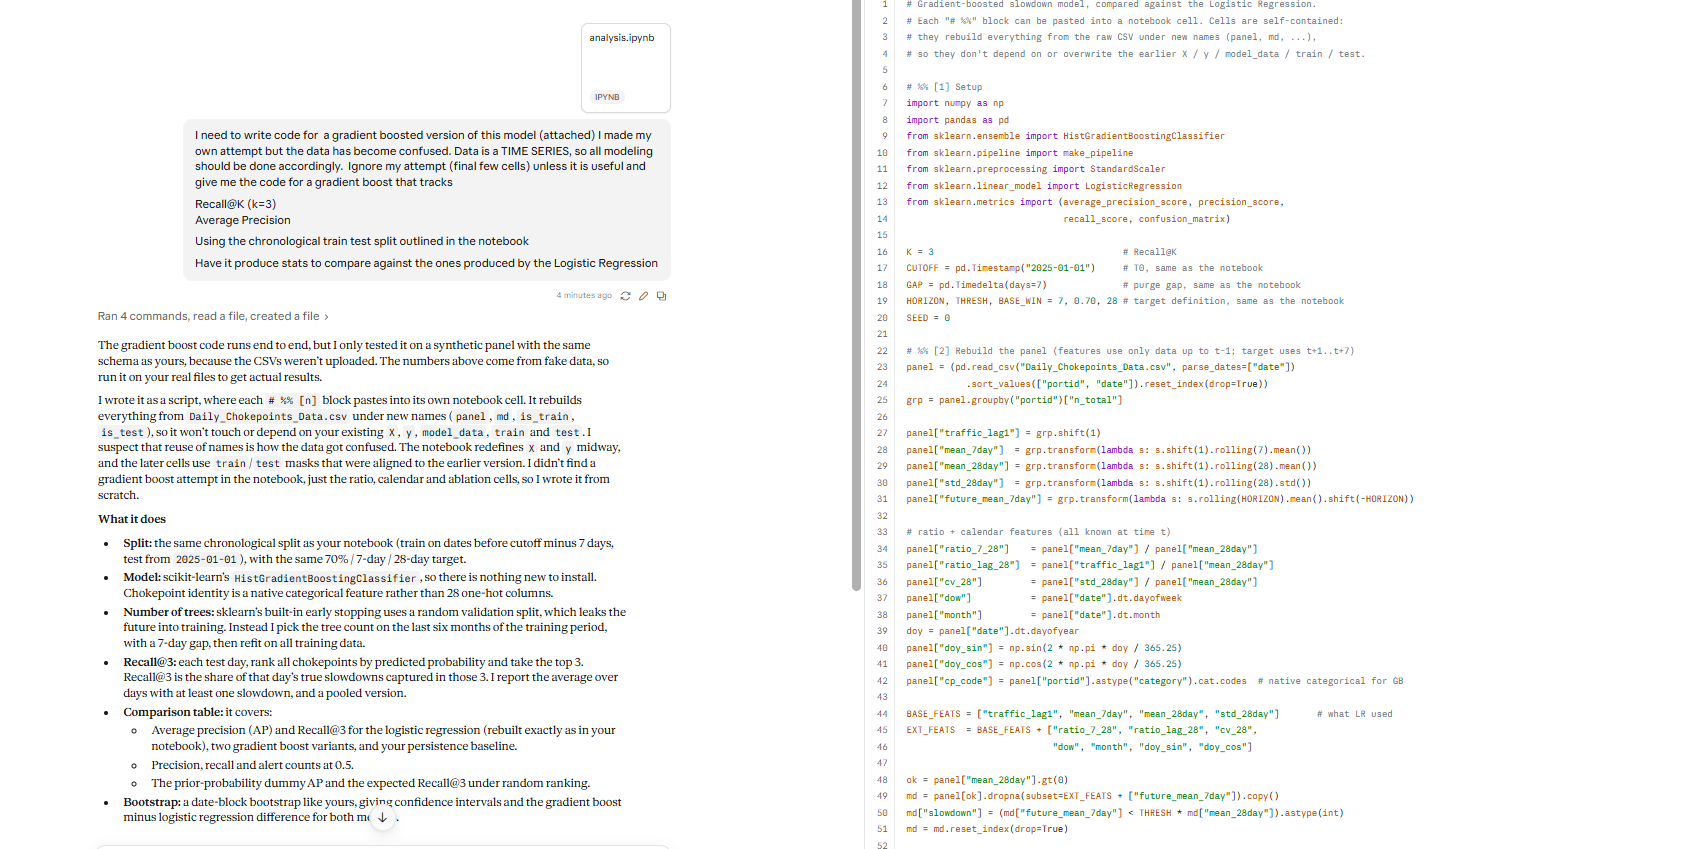
\includegraphics[width=0.8\linewidth]{Claude_1.png}
    \caption{Screenshot of request to claude for code}
    \label{fig:chokepoints}
\end{figure}
\begin{figure}[htbp]
    \centering
    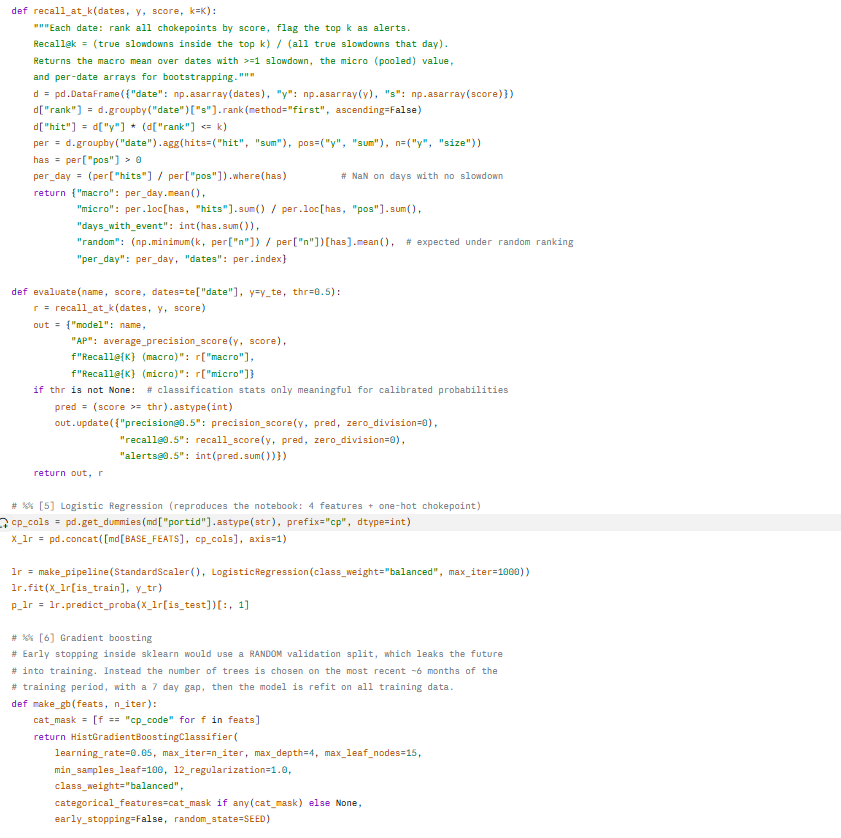
\includegraphics[width=0.8\linewidth]{Claude_2.png}
    \caption{Claude screenshot}
    \label{fig:chokepoints}
\end{figure}

\begin{figure}[htbp]
    \centering
    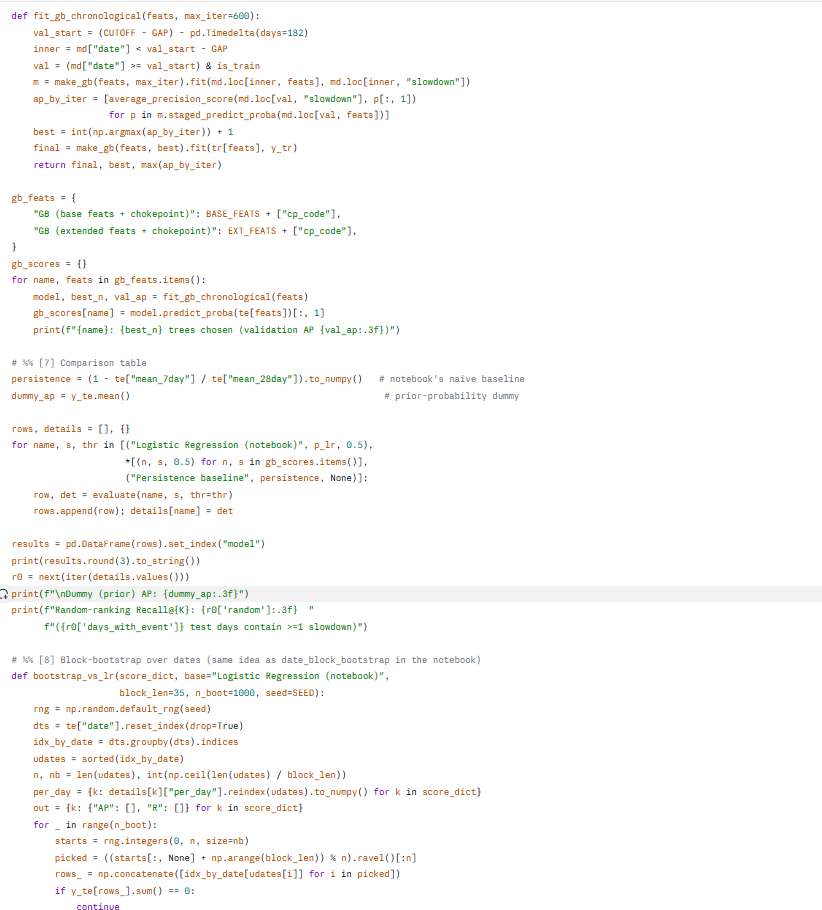
\includegraphics[width=0.8\linewidth]{Claude_3.png}
    \caption{Claude screenshot}
    \label{fig:chokepoints}
\end{figure}
\begin{figure}[htbp]
    \centering
    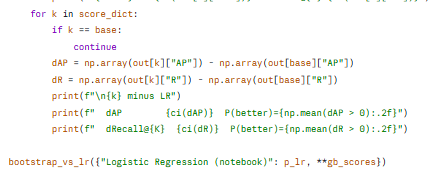
\includegraphics[width=0.8\linewidth]{Claude_4.png}
    \caption{Claude screenshot}
    \label{fig:chokepoints}
\end{figure}
% --------------------------------------------------------------------------
\begin{figure}[htbp]
    \centering
    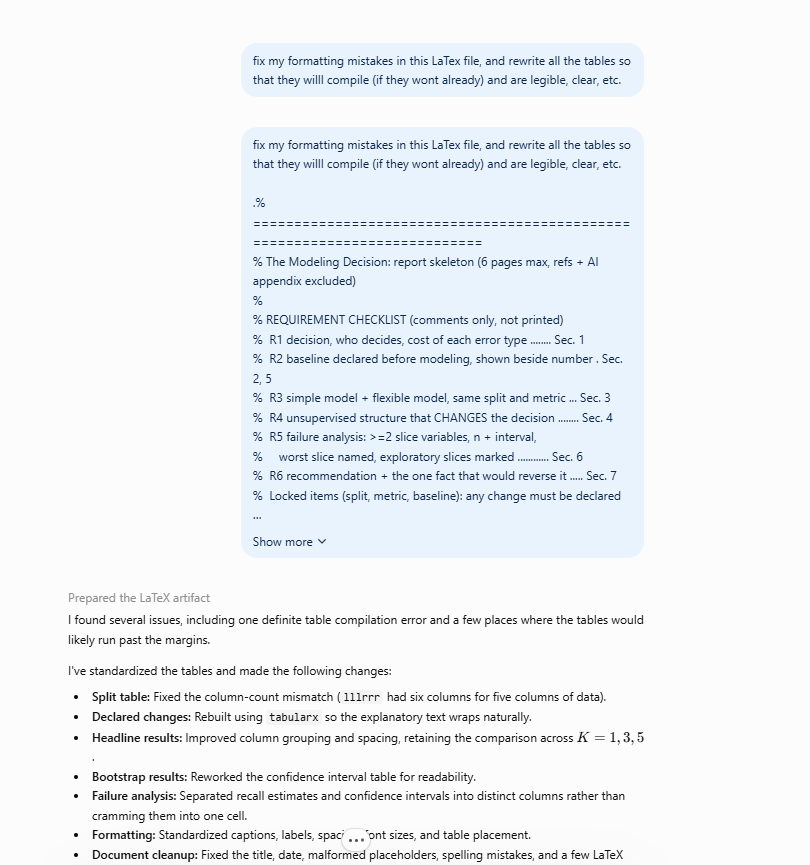
\includegraphics[width=0.8\linewidth]{ChatGPT_1.png}
    \caption{ChatGPT screenshot}
    \label{fig:chokepoints}
\end{figure}
\begin{figure}[htbp]
    \centering
    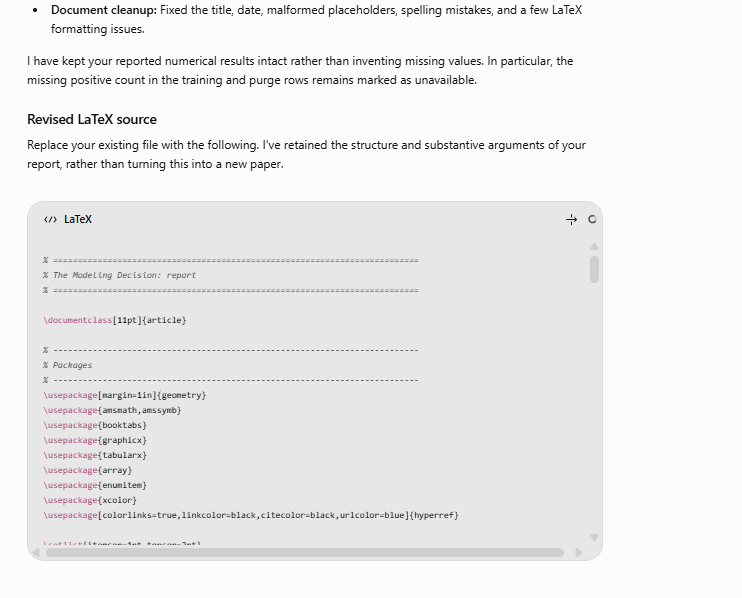
\includegraphics[width=0.8\linewidth]{ChatGPT_2.png}
    \caption{ChatGPT screenshot}
    \label{fig:chokepoints}
\end{figure}

\end{document}
